\documentclass{article}
\usepackage{tcolorbox}
\usepackage{amsmath}
\usepackage{mathtools}
\usepackage{amsfonts}
\usepackage{pgfplots}
\pgfplotsset{compat=1.16}
\usepackage[utf8]{inputenc}
\usepackage[T1]{fontenc}
\usepackage{geometry}
\geometry{
	a4paper,
	total={170mm,257mm},
	left=20mm,
	top=20mm,
}

\usepackage{tikz}

% Define the ReLU symbol command
\newcommand{\ReLU}{
	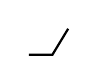
\begin{tikzpicture}[baseline=-0.5ex]
		\draw[thick] (0,-0.13) -- (0.3,-0.13) -- (0.5,0.2);
	\end{tikzpicture}
}

\begin{document}

\section{Encoder}

\begin{equation}
	X \in \mathbb{R}^{L \times D}
\end{equation}


CCA (Cross Covariance Attention): 

\begin{equation}
W_{q}^{(i)} \in \mathbb{R}^{D \times d_q}, W_{k}^{(i)} \in \mathbb{R}^{D \times d_k} \quad \forall i
\end{equation}
\begin{eqnarray}
Q^{(i)} = X W_q^{(i)} \in \mathbb{R}^{L \times d_q}, \quad K^{(i)} = X  W_k^{(i)} \in \mathbb{R}^{L \times d_k} \\
h^{(i)} = \textit{Softmax}\Bigg(\frac{(Q^{(i)})^T K^{(i)}}{\sqrt{d_{k}}}\Bigg) \in \mathbb{R}^{d_q \times d_k}
\end{eqnarray}

DHC (Dual Head Condenser):
\begin{eqnarray}
\Omega \in \mathbb{R}^{d_k \times \eta} & \zeta \in \mathbb{R}^{d_k \times 1} \\
H = h^{(1)} \Omega \in \mathbb{R}^{d_q \times \eta} & \xi = h^{(2)} \zeta \in \mathbb{R}^{d_q \times 1}
\end{eqnarray}

Final embedding:

\begin{eqnarray}
z = H^T \xi \in \mathbb{R}^{\eta \times 1}
\end{eqnarray}
\subsection{Parameters}
Number of Trainable Parameters:
\begin{eqnarray*}
\vert E_{\theta} \vert =& 2(D \times d_q) + 2(D \times d_k) + (d_k \times \eta) + (d_k \times 1) \\
=& 2Dd_{q}+2Dd_{k}+d_{k}(\eta + 1) \\
=& 2D(d_q + d_k)+d_{k}(\eta + 1)
\end{eqnarray*}

\begin{center}
\begin{figure}[h]
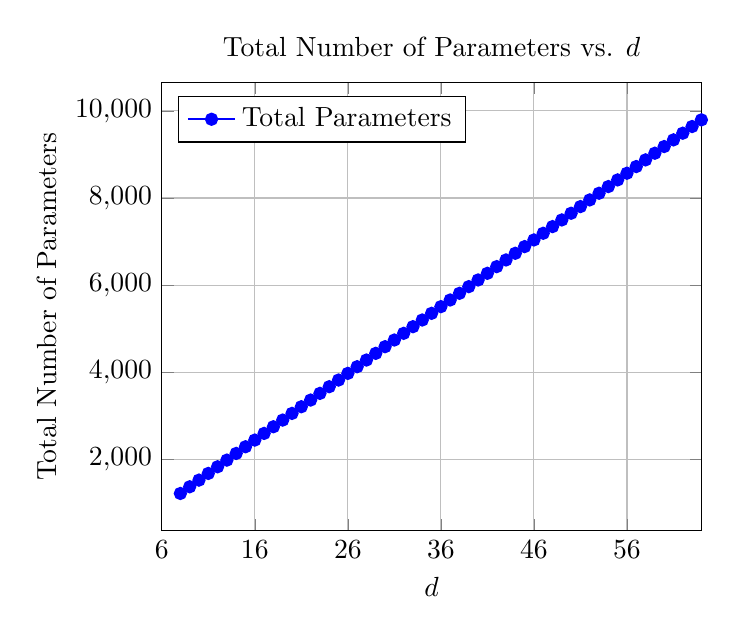
\begin{tikzpicture}
	\begin{axis}[
		title={Total Number of Parameters vs. \(d\)},
		xlabel={\(d\)},
		ylabel={Total Number of Parameters},
		grid=major,
		scaled ticks=false,
		tick label style={/pgf/number format/fixed},
		legend pos=north west,
		xmin=6, xmax=64,
		xtick={6,16,...,64} % Adding ticks at every interval of 8
	]
		
		% Calculating values within TikZ
	\addplot[
		domain=8:64,
		samples=57, % Number of d values from 8 to 64
		color=blue,
		mark=*,
		thick
	] {2*6*x + 2*6*x + x*128 + x};
	\addlegendentry{Total Parameters}
	\end{axis}
\end{tikzpicture}
\caption{Considering a case when $D = 6$ and $\eta = 128$ we assume $d_{q} = d_{k} =d$ the following plot shows how the total number of parameters vary w.r.t. $d$.}
\end{figure}
\end{center}

\section{Decoder}

Given there are $\xi$ characters in dictionary $C$ each encoded with a vector of $D$ elements.
\begin{equation}
	z \in \mathbb{R}^{\eta} \; \Rightarrow \; x \in \mathbb{R}^{\eta \times D} \quad \text{s.t.} \quad \forall x_{i} \in x \;\exists c_{i} \in C\in \mathbb{R}^{\xi \times D} \quad \text{s.t.} \vert\vert x_{i} - c_{i} \vert\vert = 0
\end{equation}
CCA (Cross Covariance Attention): 
\begin{equation}
	W_{q}^{(i)} \in \mathbb{R}^{1 \times \xi}, \quad W_{k}^{(i)} \in \mathbb{R}^{1 \times \xi}
\end{equation}

\begin{eqnarray}
	Q^{(i)} = z W_q^{(i)} \in \mathbb{R}^{\eta \times \xi}, \quad K^{(i)} = z W_k^{(i)} \in \mathbb{R}^{\eta \times \xi} \\
	h^{(i)} = \textit{Softmax}\Big((Q^{(i)})^T K^{(i)}\Big) \in \mathbb{R}^{\xi \times \xi} \\
	h_{*}^{(i)} = \textit{GumbelSoftmax}\Bigg(\textit{ReLU}\Bigg(\frac{h^{(i)}}{\sqrt{\xi}}\Bigg)\Bigg)
\end{eqnarray}

$h^{(i)}$ works as a mask matrix that when applied on $C$ it selects rows from it and constructs a new matrix $y_{i}$
\begin{equation*}
	y_{i} = h_{*}^{(i)} C \in \mathbb{R}^{\xi \times D}
\end{equation*}

\begin{tcolorbox}
	\begin{center}
		Total number of trainable parameters is $2\xi$ possibly $< \vert E_{\theta} \vert$.
	\end{center}

	\par 
	However, it is possible to create additional representation vectors for $z$ to provide surplus unknowns to the optimizer while decoding. Otherwise, if the number of unknowns in encoding, is too large compared to the number of unknowns in decoder then, it may cause incompatibility in generalization. e.g. the encoder will not use its full potential because the decoder cannot decode that.
\end{tcolorbox}

ARE (Auxiliary Representation Extraction):
\begin{equation}
	\omega_{q} \in \mathbb{R}^{1 \times \zeta}, \quad \omega_{k} \in \mathbb{R}^{1 \times \zeta}, \quad \omega_{g} \in \mathbb{R}^{2\zeta \times \zeta}
\end{equation}
\begin{eqnarray}
	q = z \omega_q \in \mathbb{R}^{\eta \times \zeta}, \quad k = \textit{Softmax}(z \omega_k) \in \mathbb{R}^{\eta \times \zeta}
\end{eqnarray}

\begin{equation}
g = \textit{Concat}\Big(q, \textit{ReLU}(k)\Big) \in \mathbb{R}^{\eta \times 2\zeta}
\end{equation}

Enriched latent space code $h$:

\begin{equation}
	h = g \omega_{g} \in \mathbb{R}^{\eta \times \zeta}
\end{equation}

Now, we pass $h$ to CCA instead of passing $z$.
\begin{equation}
	W_{q}^{(h)} \in \mathbb{R}^{\zeta \times \xi}, \quad W_{k}^{(h)} \in \mathbb{R}^{\zeta \times \xi}
\end{equation}
\begin{eqnarray}
	Q^{(h)} = h W_q^{(h)} \in \mathbb{R}^{\eta \times \xi}, \quad K^{(h)} = h W_k^{(h)} \in \mathbb{R}^{\eta \times \xi} \\
	s^{(h)} = \textit{Softmax}\Big((Q^{(h)})^T K^{(h)}\Big) \in \mathbb{R}^{\xi \times \xi} \\
	s_{*}^{(h)} = \textit{GumbelSoftmax}\Bigg(\textit{ReLU}\Bigg(\frac{s^{(h)}}{\sqrt{\xi}}\Bigg)\Bigg)
\end{eqnarray}
Finally, 
\begin{equation*}
	y_{i} = s_{*}^{(h)} C \in \mathbb{R}^{\xi \times D}
\end{equation*}

This can only generate a vector of $\xi$ elements. However we can feed this $y_{i}$ back to the decoder without causing any recursion.


\subsection{Variable sized output}

Given $X \in \mathbb{R}^{L\times D}$, where $L > \xi$, we prepare another additional vector $\overline{X} \subseteq X$ such that $\overline{X} \in \mathbb{R}^{k\xi\times D}$.

\begin{eqnarray}
	z_{1} = E_{\theta}(X) \in \mathbb{R}^{\eta} \\
	z_{2} = E_{\theta}(\overline{X}) \in \mathbb{R}^{\eta}
\end{eqnarray}

From $z_{1}, z_{2}$ we derive $Q^{(h_{1})}, K^{(h_{1})}$ and $Q^{(h_{2})}, K^{(h_{2})}$ respectively $\in \mathbb{R}^{\eta \times \xi}$.

Using trainable unknowns $\Phi ^{h_{1}} \in \mathbb{R}^{\xi \times u}$, $\Phi ^{h_{2}} \in \mathbb{R}^{\eta \times u}$ and $\Psi ^{h_{1}} \in \mathbb{R}^{\xi \times u}$, $\Psi ^{h_{2}} \in \mathbb{R}^{\eta \times u}$ we compute crossover Matrices $K^{\prime}$ and $Q^{\prime}$

\begin{center}
\begin{minipage}{\textwidth}
	\begin{center}
	\begin{minipage}{0.48\textwidth}
		\begin{eqnarray}
			K^{(h_{1})\prime} = \sigma\Bigg(\frac{K^{(h_{1})} \Phi^{(h_{1})}}{\sqrt{\xi}}\Bigg) \in \mathbb{R}^{\eta \times u} \\
			K^{(h_{2})\prime} = \sigma\Bigg(\frac{\big(K^{(h_{2})}\big)^{T} \Phi^{(h_{2})}}{\sqrt{\eta}}\Bigg) \in \mathbb{R}^{\xi \times u} \\
			K^{\prime} = \sigma\Bigg(\frac{K^{(h_{1})\prime} \Big(K^{(h_{2})\prime}\Big)^{T}}{\sqrt{u}}\Bigg)  \in \mathbb{R}^{\eta \times \xi}
		\end{eqnarray}
	\end{minipage}%
	\begin{minipage}{0.48\textwidth}
		\begin{eqnarray}
			Q^{(h_{1})\prime} = \sigma\Bigg(\frac{Q^{(h_{1})} \Psi^{(h_{1})}}{\sqrt{\xi}}\Bigg) \in \mathbb{R}^{\eta \times u} \\
			Q^{(h_{2})\prime} = \sigma\Bigg(\frac{\big(Q^{(h_{2})}\big)^{T} \Psi^{(h_{2})}}{\sqrt{\eta}}\Bigg) \in \mathbb{R}^{\xi \times u} \\
			Q^{\prime} = \sigma\Bigg(\frac{Q^{(h_{1})\prime} \Big(Q^{(h_{2})\prime}\Big)^{T}}{\sqrt{u}}\Bigg)  \in \mathbb{R}^{\eta \times \xi}
		\end{eqnarray}
	\end{minipage}
	\end{center}
\end{minipage}
\end{center}
\vspace{2mm}
Attention Matrix $S^{(h)}$

\begin{eqnarray}
	S^{(h)} = \sigma\Bigg(\frac{(Q^{\prime})^{T} K^{\prime}}{\sqrt{\xi}}\Bigg) \in \mathbb{R}^{\xi \times \xi} \\
	S^{(h)}_{*} = \sigma_{g}\Big(ReLU\big(S^{(h)}\big)\Big)
\end{eqnarray}

Finally, 
\begin{equation*}
	y_{i} = S_{*}^{(h)} C \in \mathbb{R}^{\xi \times D}
\end{equation*}

Now the output $y_{i}$ is conditioned on two inputs. One is the original input string and the other one is the part is the previous output. Therefore, we can now train it like a regular transformer model. 

\section{Modules}

\begin{tcolorbox}
	Given input $X \in \mathbb{R}^{a\times b}$ and trainable unknowns $\phi \in \mathbb{R}^{b\times r}$ \textbf{Normalized Projection Unit (NPU)} is defined as function $\mathcal{H}$.
	\begin{eqnarray*}
		\mathcal{H}(x)\vert_{\phi} \coloneqq \sigma\Bigg(\frac{X \phi}{\sqrt{b}}\Bigg) \in \mathbb{R}^{a\times r} 
	\end{eqnarray*}
\end{tcolorbox}

\begin{tcolorbox}
Given input $x \in \mathbb{R}^{L \times D}$ and trainable unknowns $\phi, \psi$, Attention and \textbf{Cross Covariance Attention (CCA)} is computed by functions $\mathcal{A}$ and $\mathcal{A}^{c}$.
	
\begin{minipage}{0.48\textwidth}
	\begin{eqnarray*}
		\begin{aligned}
		\mathcal{A}(Q,K) \coloneqq&  \sigma\Bigg(\frac{Q K^{T}}{\sqrt{u}}\Bigg) \in \mathbb{R}^{L \times L} \\
		& \text{where} \;  Q \in \mathbb{R}^{L \times u}, K \in \mathbb{R}^{L \times u}  \\
		=& \mathcal{H}(Q)\vert_{K^{T}} \\ 
		\\
		\mathcal{A}^{c}(Q,K) \coloneqq& \sigma\Bigg(\frac{Q^T K}{\sqrt{L}}\Bigg) \in \mathbb{R}^{u \times v} \\
		& \text{where} \;  Q \in \mathbb{R}^{L \times u}, K \in \mathbb{R}^{L \times v} \\
		=& \mathcal{H}(Q^{T})\vert_{K} \\
		\\
		\end{aligned}
	\end{eqnarray*}
\end{minipage}%
\begin{minipage}{0.48\textwidth}
	\begin{eqnarray*}
		\begin{aligned}
		\widehat{\mathcal{A}}(x)\vert_{\phi, \psi} \coloneqq& \mathcal{A}(x\phi, x\psi) \in \mathbb{R}^{L \times L} \\
		& \text{where} \; \phi \in \mathbb{R}^{D\times u}, \psi \in \mathbb{R}^{D \times u} \\
		\\
		\\
		\\
		\\
		\\
		\widehat{\mathcal{A}^{c}}(x)\vert_{\phi, \psi} \coloneqq& \mathcal{A}^{c}(x\phi, x\psi) \in \mathbb{R}^{u \times v} \\
		& \text{where} \; \phi \in \mathbb{R}^{D\times u}, \psi \in \mathbb{R}^{D \times v} \\
		\\
		\end{aligned}
	\end{eqnarray*}
\end{minipage}
\end{tcolorbox}

\begin{tcolorbox}
	Given $h_{1}, h_{2} \in \mathbb{R}^{u\times v}$ and trainable unknowns $\omega \in \mathbb{R}^{v\times \eta}, \xi \in \mathbb{R}^{v\times 1}$, \textbf{Dual Head Compressor (DHC)} $\Omega$
	
	\begin{equation*}
		\Omega(h_{1}, h_{2}) \coloneqq (h_{1} \omega)^{T} (h_{2}\xi) \in \mathbb{R}^{\eta}
	\end{equation*}
\end{tcolorbox}

\begin{tcolorbox}
Given $m_{1}, m_{2} \in \mathbb{R}^{\eta \times \zeta}$, $\phi\in \mathbb{R}^{\zeta\times u}$, $\psi \in \mathbb{R}^{\eta\times u}$  \textbf{Feature Crossover Covariance (FCC)} function $\Gamma$
\begin{eqnarray*}
	\begin{aligned}
	\Gamma(m_{1}, m_{2})\vert_{\phi, \psi} \coloneqq& \sigma\Bigg(\frac{\mathcal{H}(m_{1})\vert_{\phi} \Big(\mathcal{H}(m_{2}^{T})\vert_{\psi}\Big)^{T} }{\sqrt{u}}\Bigg) \in \mathbb{R}^{\eta\times \zeta} \\
	=& \mathcal{A}(\mathcal{H}(m_{1})\vert_{\phi}, \mathcal{H}(m_{2}^{T})\vert_{\psi})
	\end{aligned}
\end{eqnarray*}
\end{tcolorbox}


\begin{tcolorbox}
Given $x_{1}, x_{2} \in \mathbb{R}^{\eta \times \tau}$, $\omega^{(q)}_{i} \in \mathbb{R}^{\tau \times \zeta}$, $\omega^{(k)}_{i} \in \mathbb{R}^{\tau \times \zeta}$ and $\phi^{(q)}, \phi^{({k})} \in \mathbb{R}^{\zeta \times u}$, $\psi^{(q)}, \psi^{({k})} \in \mathbb{R}^{\eta \times u}$. \textbf{Cross Crossover Covariance Attention (CCCA)} is computed by function $\Upsilon$.
\begin{eqnarray*}
	\begin{aligned}
	\Upsilon(x_{1}, x_{2})\vert_{\omega^{(q)}, \omega^{(k)}}\coloneqq&\mathcal{A}^{c}(Q^{\prime}, K^{\prime}) & \in \mathbb{R}^{\zeta\times \zeta} \\
	& \text{where} & Q^{\prime} = \Gamma\Big(x_{1} \omega^{(q)}_{1}, x_{2} \omega^{(q)}_{2}\Big) \vert_{\phi^{(q)}, \psi^{(q)}} \in \mathbb{R}^{\eta\times \zeta} \\
	& & K^{\prime} = \Gamma\Big(x_{1} \omega^{(k)}_{1}, x_{2} \omega^{(k)}_{2}\Big) \vert_{\phi^{(k)}, \psi^{(k)}} \in \mathbb{R}^{\eta\times \zeta}
	\end{aligned}
\end{eqnarray*}
\begin{eqnarray*}
	\begin{aligned}
	\widehat{\Upsilon}(x_{1}, x_{2})\vert_{\omega^{(q)}, \omega^{(k)}}\coloneqq& \sigma_{g}(\ReLU(\Upsilon(x_{1}, x_{2})\vert_{\omega^{(q)}, \omega^{(k)}})) &
	\end{aligned}
\end{eqnarray*}
\end{tcolorbox}

\begin{tcolorbox}

Given input $X \in \mathbb{R}^{n \times 1}$ and trainable unknowns $\beta \in \mathbb{R}^{1 \times \tau}, s \in \mathbb{R}^{1 \times \tau}, \mu \in \mathbb{R}^{2\tau \times \tau}$, \textbf{Auxiliary Enriched Augmentation (AEA)} $\Lambda$.

\begin{equation*}
	\Lambda(X) \coloneqq \textit{Cat}(X_{\beta}, \ReLU(X_{s}))\mu \in \mathbb{R}^{n\times \tau} \quad \text{where}\; X_{\beta} = x \beta \in \mathbb{R}^{n \times \tau}, \quad X_{s} = \sigma(X s) \in \mathbb{R}^{n \times \tau}
\end{equation*}
\end{tcolorbox}

\subsection{Encoding}
\begin{minipage}{0.3\textwidth}
\begin{eqnarray*}
	x \xrightarrow[w_{q}^{(1)}, w_{k}^{(1)}]{\widehat{\mathcal{A}^{c}}} h_{1} \\
	x \xrightarrow[w_{q}^{(2)}, w_{k}^{(2)}]{\widehat{\mathcal{A}^{c}}} h_{2} \\
	x \xrightarrow[w_{q}^{(3)}, w_{k}^{(3)}]{\widehat{\mathcal{A}^{c}}} h_{3} \\
	\vdots \\
	x \xrightarrow[w_{q}^{(n)}, w_{k}^{(n)}]{\widehat{\mathcal{A}^{c}}} h_{n}
\end{eqnarray*}
\end{minipage}%
\begin{minipage}{0.3\textwidth}
	\begin{eqnarray*}
		(h_{1}, h_{2})& \xrightarrow[\omega_{1}, \xi_{1}]{\Omega}& H_{1} \\
		(h_{2}, h_{3})& \xrightarrow[\omega_{2}, \xi_{2}]{\Omega}& H_{2} \\
		& \vdots \\
		(h_{n-1}, h_{n})& \xrightarrow[\omega_{n-1}, \xi_{n-1}]{\Omega}&  H_{n-1}
	\end{eqnarray*}
\end{minipage}%
\begin{minipage}{0.3\textwidth}
	\begin{eqnarray*}
		H = \frac{1}{N}\sum_{i}^{N-1} H_{i}
	\end{eqnarray*}
\end{minipage}

\subsection{Decoding}
\begin{minipage}{0.3\textwidth}
\begin{eqnarray*}
	z_{1}\in \mathbb{R}^{\eta} \xrightarrow[\beta, s, \mu]{\Lambda} h_{1} \in \mathbb{R}^{\eta\times \tau } \\
	z_{2}\in \mathbb{R}^{\eta} \xrightarrow[\beta, s, \mu]{\Lambda} h_{2}\in \mathbb{R}^{\eta\times \tau }
\end{eqnarray*}
\end{minipage}%
\begin{minipage}{0.3\textwidth}
	\begin{eqnarray*}
		(h_{1}, h_{2})\xrightarrow[\omega^{(q)}, \omega^{(k)}, \phi^{(q)}, \psi^{(k)}]{\widehat{\Upsilon}} y \in \mathbb{R}^{\zeta\times \zeta}
	\end{eqnarray*}
\end{minipage}%
\begin{minipage}{0.3\textwidth}
	\begin{eqnarray*}
		yC\in \mathbb{R}^{\zeta\times D}
	\end{eqnarray*}
\end{minipage}

%\subsection{Encoder}
%$E: X \rightarrow Z$ where $X \in \mathbb{R}^{L\times D}$, $Z \in \mathbb{R}^{\eta}$
%
%Trainable Parameters: (Number of heads $N_{h} > 1$)
%\begin{eqnarray*}
%w_{q}^{(i)} \in \mathbb{R}^{D \times d_q}, w_{k}^{(i)} \in \mathbb{R}^{D \times d_k} \quad &\forall i < N_{h} \\
%w_{m}^{(i)} \in \mathbb{R}^{d_k \times \eta}, w_{t}^{(i)} \in \mathbb{R}^{d_k \times 1} \quad &\forall i < N_{h}-1 
%\end{eqnarray*}
%
%pipeline:
%
%\begin{eqnarray*}
%	\begin{aligned}
%	z = E(x) \coloneqq& \frac{1}{N_{h}-1} \sum\limits_{i}^{N_{h}-1} z_{i} & \in \mathbb{R}^{\eta \times 1} \\
%	z_{i} =& \Big(H_{m}^{(i)}\Big)^{T}\Big(H_{t}^{(i)}\Big) &\in \mathbb{R}^{\eta \times 1} \\
%	H_{t}^{(i)} =& h^{(i+1)}w_{t}^{(i)} &\in \mathbb{R}^{d_q \times 1} \\
%	H_{m}^{(i)} =& h^{(i)}w_{m}^{(i)} &\in \mathbb{R}^{d_q \times \eta} \\
%	h^{(i)} =& \mathcal{A}^{c}(x)\vert_{w_{q}^{(i)}, w_{k}^{(i)}} &\in \mathbb{R}^{d_q \times d_k}
%	\end{aligned}
%\end{eqnarray*}
%
%\subsection{Decoder}
%$E: Z \times Z \rightarrow X$ where $X \in \mathbb{R}^{L\times D}$, $Z \in \mathbb{R}^{\eta}$
%
%Trainable Parameters:
%\begin{eqnarray*}
%	b\in \mathbb{R}^{1\times \tau}, b^{\prime}\in \mathbb{R}^{1\times \tau}, c\in \mathbb{R}^{2\tau \times \tau}
%\end{eqnarray*}
%
%pipeline:
%
%\begin{eqnarray*}
%	\begin{aligned}
%		z_{1}^{(Q)} = \mathcal{H}(z_{1}^{(\beta)} \omega_{q})\vert_{\Phi,\Psi}\\
%		z_{1}^{(K)} = \mathcal{H}(z_{1}^{(\beta)} \omega_{k})\vert_{\Phi,\Psi}\\
%		z_{2}^{(Q)} = \mathcal{H}(z_{1}^{(\beta)} \omega_{q})\vert_{\Phi,\Psi}\\
%		z_{2}^{(K)} = \mathcal{H}(z_{1}^{(\beta)} \omega_{k})\vert_{\Phi,\Psi}\\
%		z_{1}^{(\beta)} = \mathcal{\beta}_{\tau}(z_{1})\vert_{b, b^{\prime},c} \in \mathbb{R}^{\eta \times \tau} \\
%		z_{2}^{(\beta)} = \mathcal{\beta}_{\tau}(z_{2})\vert_{b, b^{\prime},c} \in \mathbb{R}^{\eta \times \tau} \\
%	\end{aligned}
%\end{eqnarray*}

\end{document}
